\begin{multicols}{2}

\noindent (тут, конечно, нам повезло: разность квадратов 

\noindent $(2n + 1)^2 - 4n(n + 1)$ равна 1.

\noindent$\leq \frac {i}{(2\sqrt{n\mathstrut} \ + \sqrt{n\mathstrut} \ + \sqrt{n\mathstrut})\ (2n + 2n)} = \frac1{16n\sqrt{n\mathstrut}}$.

\bigskip

\scriptsize Заметим, что и эта оценка очень точная. Но убедиться в этом (и вообще исследовать поведение функции с многими радикалами) лучше уже 
не с помощью алгебраических преобразований, а средствами анализа - заменить переменную n на h 1/n и вопспользоваться формулой Тейлора
$\sqrt{1+h\mathstrut} - 1 + h/2 - h^2/8 + ...$ (См. [6].)
\normalsize
\bigskip\bigskip\bigskip\bigskip

\noindent \textbf{Заменим плюс на минус}

\medskip
\noindent Мы уже говорили о пользе симметрии в геометрических задачах. Своего рода
симметрией в \so{алгебре} является замена плюса на минус.

Так, если какое-либо выражение от
$\sqrt{d\mathstrut}$ равно $p+q\sqrt{d\mathstrut}$ и мы всюду в этом
выражении заменим $\sqrt{d\mathstrut}$ на $-\sqrt{d\mathstrut}$, то
естественно ожидать, что новое выражение окажется равным сопряженному числу $p-q\sqrt{d\mathstrut}$. Мы будем пользоваться таким очевидным частным случаем этого 
свойства (a и b - рациональны, $\sqrt{d\mathstrut}$ -
нет):

\medskip
\noindent $(a + b\sqrt{d\mathstrut})^n = p + q\sqrt{d\mathstrut}$ $\Rightarrow$
\medskip

\leftskip=1cm
$\Rightarrow$ $(a - b\sqrt{d\mathstrut})^n = p - q\sqrt{d\mathstrut}$.

\leftskip=0cm
\smallskip

\textbf{5.} \textit{Доказать, что уравнение}
\[
(x + y\sqrt{5\mathstrut})^4 + (z + t\sqrt{5\mathstrut})^4 = 2 + \sqrt{5\mathstrut} \tag{4}
\]

\noindent \textit{не имеет решений в рациональных числах}

\noindent \textit{x, y, z, t.}

Можно, конечно, найти отдельно сумму
членов левой части, не содержащих $\sqrt{5\mathstrut}$
(она должна быть равна 2), и отдельно "---
коэффициент при $\sqrt{5\mathstrut}$ (он должен 
равняться 1). Но что делать с полученной
громаздкой системой, неясно. 
Вместо этого воспользуемся (4) и заменим
плюс перед $\sqrt{5\mathstrut}$ на минус!
\[
(x - y\sqrt{5\mathstrut})^4 + (z - t\sqrt{5\mathstrut})^4 = 2 - \sqrt{5\mathstrut}
\]

\noindent Слева стоит неотрицательное число, справа 
"--- отрицательное.

\textbf{6.} \textit{Доказать, что существует бесконечно много пар (x; y) натуральных чисел, 
для которых $x^2$ отличается от $2y^2$ на 1:}

\[
  |x^2 - 2y^2| = 1 \tag{5}
\]

Несколько таких пар с небольшим
(x; y) легко найти подбором: это (1; 2), 
(3;2), (7,5), (17,12),...(рис. 1). Как 
продолжить этот набор? Можно ли запиcать общую формулу для этих решений?
\begin{flushleft}
    \textbf{28}
\end{flushleft}
\columnbreak
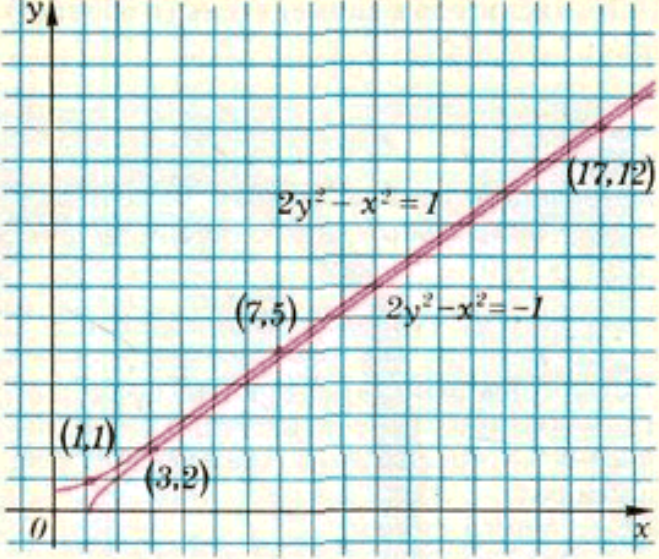
\includegraphics[height=75mm,width=95mm]{kvant_pic1.png}

\noindent \textbf{Рис. 1. Проходят ли эти гиперболы через бесконечное число узлов клетчатой бумаги?}
\bigskip

Найти ответы на эти вопросы нам поможет
число $1 + \sqrt{2\mathstrut}$. Закономерность, позволяющая получать все новые и новые решения (x; y), указана в таблице:

\scriptsize
\bigskip
\noindent \begin{tabular}{|c|c|c|c|c|c|}
    \hline
    n & $(1 + \sqrt{2\mathstrut})^n$ & $x_n$ & $y_n$ & $(x_n)^2 - 2(y_n)^2$ & $(1 - \sqrt{2\mathstrut})^n$ \\ [2.5ex]
    \hline
    1 & $1 + \sqrt{2\mathstrut}$ & 1 & 1 & $1 - 2 = -1$ & $1 - \sqrt{2\mathstrut}$ \\
    2 & $3 + 2\sqrt{2\mathstrut}$ & 3 & 2 & $9 - 8 = 1$ & $3 - 2\sqrt{2\mathstrut}$ \\
    3 & $7 + 5\sqrt{2\mathstrut}$ & 7 & 5 & $49 - 50 = -1$ & $7 - 5\sqrt{2\mathstrut}$ \\
    4 & $17 + 12\sqrt{2\mathstrut}$ & 17 & 12 & $289 - 288 = 1$ & $17 - 12\sqrt{2\mathstrut}$ \\
    5 & $41 + 29\sqrt{2\mathstrut}$ & 41 & 29 & $1681 - 1682 = -1$ & $41 - 29\sqrt{2\mathstrut}$ \\[2.5ex]
    .. & ... & .. & .. & .... & .....\\[2.5ex]
    \hline
\end{tabular}

\smallskip
\normalsize

\noindent \textbf{Какой будет шестая строчка?}
\smallskip

\noindent Видно, что коэффициенты $x_n$, $y_n$ в числе
\[
    x_n + y_n\sqrt{2\mathstrut} = (1 + \sqrt{2\mathstrut})^n
\]
будут давать нужную пару. Доказать это 
поможет колонка таблицы из сопряженных
чисел (мы снова применяем (4)):
\[
    x_n - y_n\sqrt{2\mathstrut} = (1 - \sqrt{2\mathstrut})^n
\]
Перемножив два последних равенства, получим
\smallskip

\noindent $x_n^2 - 2y_n^2 = (1 + \sqrt{2\mathstrut})^n(1 - \sqrt{2\mathstrut})^n = $ 
\smallskip

$=((1 + \sqrt{2\mathstrut})(1 - \sqrt{2\mathstrut}))^n = (-1)^n$,
\smallskip

\noindent и интересующее нас выражение попеременно 
равно то 1, то -1. Складывая и вычитая эти 
же два равенства, мы получим явное 
выражение для $x_n$ и $y_n$:
\smallskip

$x_n = ((1 + \sqrt{2\mathstrut})^n + (1 - \sqrt{2\mathstrut})^n)/2$

$y_n = ((1 + \sqrt{2\mathstrut})^n - (1 - \sqrt{2\mathstrut})^n)/2\sqrt{2\mathstrut}$.

\end{multicols}
